% !TEX program = xelatex
\documentclass[10pt]{article}

% ==========================================================================
% VARIÁVEL DE COR DO CURRÍCULO
% Altere apenas o código hexadecimal abaixo (sem '#') conforme a empresa
% (ex.: b88324 padrão dourado | EA1D2C vermelho oficial iFood):
% ==========================================================================
\providecommand{\CorEmpresa}{2f804c}

% ==========================================================================
% PACOTES E CONFIGURAÇÃO DE PÁGINA (1 PÁGINA A4)
% ==========================================================================
\usepackage[
  paperwidth=595.5bp,
  paperheight=842.25bp,
  left=23bp,
  right=23bp,
  top=21bp,
  bottom=20bp
]{geometry}
\usepackage{fontspec}
\usepackage{xcolor}
\usepackage{tikz}
\usepackage{enumitem}
\usepackage[normalem]{ulem}
\usepackage{ragged2e}
\usepackage{calc}
\usepackage[
  colorlinks=true,
  linkcolor=accent,
  urlcolor=accent
]{hyperref}

\definecolor{accent}{HTML}{\CorEmpresa}

\pagestyle{empty}
\frenchspacing
\setlength{\parindent}{0pt}
\setlength{\parskip}{0pt}

% Desabilita hifenização automática para manter leitura limpa
\hyphenpenalty=10000
\exhyphenpenalty=10000
\tolerance=2000
\emergencystretch=3em

% ==========================================================================
% FONTES (com fallback seguro caso alguma fonte não esteja instalada)
% ==========================================================================
\IfFontExistsTF{Arial}{
  \setmainfont{Arial}[
    LetterSpace=2.0,
    WordSpace={1.05,1.80,0.45},
    BoldFont={Arial Bold},
    ItalicFont={Arial Italic},
    BoldItalicFont={Arial Bold Italic}
  ]
}{
  \setmainfont{TeX Gyre Heros}[
    LetterSpace=2.0,
    WordSpace={1.05,1.80,0.45}
  ]
}

\IfFontExistsTF{Libre Baskerville}{
  \newfontfamily\BaskervilleItalic{Libre Baskerville}[
    LetterSpace=3.5,
    WordSpace=1.12,
    UprightFont={* Italic},
    ItalicFont={* Italic}
  ]
  \newfontfamily\BaskervilleSection{Libre Baskerville}[
    LetterSpace=18.0
  ]
}{
  \newfontfamily\BaskervilleItalic{BaskervilleF}[
    LetterSpace=3.5,
    WordSpace=1.12,
    UprightFont={*-Italic},
    ItalicFont={*-Italic}
  ]
  \newfontfamily\BaskervilleSection{BaskervilleF}[
    LetterSpace=18.0
  ]
}

\IfFileExists{fonts/RedHatDisplay-Regular.ttf}{
  \newfontfamily\ContactFont{RedHatDisplay-Regular.ttf}[
    Path=fonts/,
    LetterSpace=3.0,
    WordSpace=1.12
  ]
}{
  \IfFontExistsTF{Red Hat Display}{
    \newfontfamily\ContactFont{Red Hat Display}[
      LetterSpace=3.0,
      WordSpace=1.12
    ]
  }{
    \newfontfamily\ContactFont{Arial}[
      LetterSpace=3.0,
      WordSpace=1.12
    ]
  }
}

% ==========================================================================
% LINKS SUBLINHADOS NA COR DA EMPRESA (permite quebra de linha)
% ==========================================================================
\newcommand{\accentuline}{%
  \bgroup\markoverwith{\textcolor{accent}{\rule[-1.6bp]{1bp}{0.65bp}}}\ULon
}
\newcommand{\cvlink}[2]{%
  \href{#1}{{\color{accent}\accentuline{#2}}}%
}

% ==========================================================================
% MACROS DE ESTRUTURA DO CURRÍCULO
% ==========================================================================
\newsavebox{\cvbulletbox}
\AtBeginDocument{\sbox{\cvbulletbox}{\tikz\fill[black] (0,0) circle (1.35bp);}}

% Título de seção com seta horizontal em TikZ na cor \CorEmpresa
\newcommand{\cvsection}[1]{%
  \par\vspace{5.0bp}%
  \noindent{\BaskervilleSection\fontsize{8.8bp}{10.0bp}\selectfont #1}\par
  \vspace{-5.6bp}%
  \noindent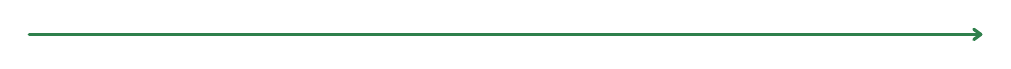
\begin{tikzpicture}[baseline=(current bounding box.north)]
    \draw[accent, line width=1.15bp, line cap=round, line join=round] (0.58bp,0) -- (\textwidth-0.58bp,0);
    \draw[accent, line width=1.15bp, line cap=round, line join=round] (\textwidth-3.1bp,1.85bp) -- (\textwidth-0.58bp,0) -- (\textwidth-3.1bp,-1.85bp);
  \end{tikzpicture}\par
  \vspace{2.5bp}%
}

% Entrada de experiência ou formação acadêmica
% #1 = Título/Cargo (negrito, cor accent)
% #2 = Período (itálico, alinhado à direita)
% #3 = Instituição/Empresa (itálico, esquerda)
% #4 = Localidade ou GPA (direita)
\newcommand{\cventry}[4]{%
  \par\noindent
  {\fontsize{7.95bp}{9.0bp}\selectfont
  \makebox[\textwidth][s]{\textbf{\textcolor{accent}{#1}}\hfill\textit{#2}}\par
  \makebox[\textwidth][s]{\textit{#3}\hfill #4}\par}%
}

% Espaço entre entradas consecutivas
\newcommand{\entrygap}{\vspace{3.0bp}}

% Lista de bullets padrão (círculo sólido, texto justificado)
\newlist{cvbullets}{itemize}{1}
\setlist[cvbullets,1]{
  label={\raisebox{1.85bp}{\usebox{\cvbulletbox}}},
  leftmargin=11.8bp,
  rightmargin=0.8bp,
  labelwidth=3.2bp,
  labelsep=4.8bp,
  itemindent=0bp,
  topsep=0bp,
  partopsep=0bp,
  parsep=0bp,
  itemsep=0.3bp,
  before={\justifying\fontsize{7.75bp}{9.05bp}\selectfont}
}
\AddToHook{env/cvbullets/begin}{\vspace{-1.1bp}}

% Lista de publicações / conquistas
\newlist{cvpublist}{itemize}{1}
\setlist[cvpublist,1]{
  label={\raisebox{1.85bp}{\usebox{\cvbulletbox}}},
  leftmargin=11.8bp,
  rightmargin=0.8bp,
  labelwidth=3.2bp,
  labelsep=4.8bp,
  itemindent=0bp,
  topsep=0bp,
  partopsep=0bp,
  parsep=0bp,
  itemsep=0.4bp,
  before={\justifying\fontsize{7.75bp}{9.05bp}\selectfont}
}
\AddToHook{env/cvpublist/begin}{\vspace{-0.4bp}}

% ==========================================================================
% DOCUMENTO (1 PÁGINA)
% ==========================================================================
\begin{document}

% --- CABEÇALHO ---
\noindent
\begin{minipage}[b]{0.72\textwidth}
  {\BaskervilleItalic\fontsize{19.0bp}{20.0bp}\selectfont João Victor Assaoka Ribeiro}
\end{minipage}%
\hfill
\begin{minipage}[b]{0.27\textwidth}
  \raggedleft
  \lineskiplimit=-10bp
  \BaskervilleItalic\fontsize{10.5bp}{10.8bp}\selectfont Generative AI\\Engineer\par
\end{minipage}

\vspace{3.0bp}

% --- CONTATOS ---
{\centering\ContactFont\fontsize{8.0bp}{8.8bp}\selectfont
\cvlink{https://api.whatsapp.com/send?phone=5531997000405}{(31) 99700-0405} ·
\cvlink{mailto:joao.assaoka@unifesp.br}{joao.assaoka@unifesp.br} ·
Portfolio: \cvlink{https://assaoka.com/}{assaoka.com} ·
GitHub: \cvlink{https://github.com/Assaoka}{github.com/Assaoka} · \\
LinkedIn: \cvlink{http://www.linkedin.com/in/assaoka}{linkedin.com/in/assaoka} ·
Hugging Face: \cvlink{https://huggingface.co/Assaoka}{huggingface.co/Assaoka} ·
Google Scholar: \cvlink{https://scholar.google.com/citations?user=4XKCFF4AAAAJ}{4XKCFF4AAAAJ}\par}

\vspace{3.0bp}

% --- HARD SKILLS, SOFT SKILLS & LANGUAGES ---
{\justifying\fontsize{7.75bp}{9.0bp}\selectfont
\noindent\textbf{Hard Skills.} Python, SQL, SQLAlchemy, Software Engineering, Object-Oriented Programming (OOP), APIs, FastAPI, LLMs, Generative AI, AI Agents, Multi-Agent Systems, Agent Architecture, Prompt Engineering, Text-to-SQL, LangChain, LangGraph, Hugging Face, LLM Evaluation, Automated Testing, Machine Learning, Deep Learning, Explainable AI (XAI), Data Engineering, Scientific Research, Kaggle, Streamlit, Selenium, Linux, HPC, Slurm, Claude Code, Antigravity\par
\vspace{0.8bp}
\noindent\textbf{Soft Skills.} Leadership, Project Management, Cross-Functional Teamwork, Problem Solving, Autonomy, Assertiveness, Continuous \& Fast Learning, Growth Mindset, Clear Technical Communication, Didactics, Training Delivery, Workshop Facilitation, Conference Presentations\par
\vspace{0.8bp}
\noindent\textbf{Languages.} Portuguese (Native), English (Advanced)\par}

% --- EDUCATION ---
\cvsection{EDUCATION}

\cventry{PhD in Computer Science (Direct Track, Special Student)}{Mar 2024 - Present}{Federal University of São Paulo (UNIFESP)}{GPA: \textbf{A}}
\begin{cvbullets}
  \item Completed graduate-level coursework concurrently with undergraduate studies.
\end{cvbullets}

\entrygap
\cventry{Visiting International Research Student (VIRS)}{May 2026 - Aug 2026}{Dalhousie University}{Halifax, Canada}

\entrygap
\cventry{B.S. in Computer Science (BCC)}{Feb 2026 - Present}{Federal University of São Paulo (UNIFESP)}{GPA: \textbf{9.25/10}}
\begin{cvbullets}
  \item Ranked 3rd in the interdisciplinary bachelor's degree progression selection process.
\end{cvbullets}

\entrygap
\cventry{B.S. in Interdisciplinary Science and Technology (BICT)}{Mar 2023 - Feb 2026}{Federal University of São Paulo (UNIFESP)}{GPA: \textbf{9.23/10}}
\begin{cvbullets}
  \item Certificate of Emphasis in Data Science Fundamentals.
\end{cvbullets}

% --- PROFESSIONAL EXPERIENCE ---
\cvsection{PROFESSIONAL EXPERIENCE}

\cventry{Natural Language Processing Researcher}{Nov 2024 - Present}{PARANA Research Group | FAPESP | Serasa Experian}{Remote}
\begin{cvbullets}
  \item Increased correlation with human judgment from 0.23 to 0.49 in news summarization quality evaluation by proposing task decomposition with LLMs in LangChain.
  \item Accelerated the multi-task retraining cycle from 1h17min to 25s while preserving 94.7\% of Macro-F1 by architecting a Model Merging strategy for SLMs via Mergekit.
  \item Improved Macro-F1 by 31.2\% relative in multi-class toxicity detection under imbalanced scenarios by structuring synthetic data augmentation pipelines via LLMs.
  \item Built a proprietary financial-domain dataset, developing web scraping via Selenium, the annotation platform in Streamlit, relational modeling in PostgreSQL (Neon/SQLAlchemy), and exploratory analysis with Pandas and Matplotlib.
  \item Architected fine-tuning (Full, LoRA, IA3, Soft Prompts via Hugging Face) and inference (vLLM) pipelines with structured outputs, orchestrating experiments on multi-GPU NVIDIA nodes in a Linux HPC environment (Digital Research Alliance of Canada) via Slurm.
\end{cvbullets}

\entrygap
\cventry{Supervisor / Manager of Data and AI}{Dec 2024 - Jan 2026}{SciTec Jr.}{Remote}
\begin{cvbullets}
  \item Founded the consultancy's dedicated Data Science and Artificial Intelligence department, leading the spin-off from the computing area and new recruitment criteria that enabled attracting talent across multiple Engineering programs at UNIFESP.
  \item Managed the delivery of 6 projects, comprising 3 consulting initiatives for external clients and 3 internal operational automation products.
  \item Trained new consultants in Data and AI competencies.
\end{cvbullets}

\entrygap
\cventry{Generative AI Engineer}{Feb 2025 - Jul 2025}{Ativamente - Enactus UNIFESP São José dos Campos}{Remote}
\begin{cvbullets}
  \item Developed a conversational Text-to-SQL agent capable of interpreting natural language queries and extracting analytical metrics on demand. \cvlink{https://www.linkedin.com/posts/assaoka_impactosocial-inteligenciaartificial-datascience-ugcPost-7376608320402554880-8AZP/?utm_source=share&utm_medium=member_desktop&rcm=ACoAAEyn-X4Bum6lMYdO9wfc_GieQOxCXYj2FIA}{Video demonstration}.
  \item Reduced clinical report generation time from over 1–3 hours to 5 minutes by architecting an integrated data solution with Streamlit and automated LLM summarization.
  \item Centralized and standardized the workshops' data ecosystem, replacing fragmented legacy spreadsheets with a structured relational architecture and input forms.
\end{cvbullets}

\entrygap
\cventry{Prescriptive Maintenance \& XAI Researcher}{Jul 2023 - Dec 2024}{PARANA Research Group | FAPESP | IAsmin Platform | Siemens Energy}{Remote}
\begin{cvbullets}
  \item Enabled cost savings and industrial failure prevention by predicting degradation signals in time series, developing models from baselines (Linear Regression) to ensembles (XGBoost) and deep recurrent architectures (LSTM).
  \item Implemented an Explainable Artificial Intelligence (XAI) framework using SHAP, ALE, and PDP plots, diagnosing causal interactions to validate alignment of predictions with domain knowledge and increase decision-making transparency.
  \item Created the \cvlink{https://blog-ia-unifesp.vercel.app/}{IAsmin educational platform}, democratizing XAI and Industry 4.0 predictive maintenance practices by publishing 7 practical tutorials detailing conceptual foundations and technical implementation.
\end{cvbullets}

% --- PUBLISHED PAPERS ---
\cvsection{PUBLISHED PAPERS}

\begin{cvpublist}
  \item \cvlink{https://sol.sbc.org.br/index.php/eniac/article/view/47030}{United Experts: Efficient Multi-Task Sentiment Analysis in Portuguese via Model Merging} - XXIII Encontro Nacional de Inteligência Artificial e Computacional (ENIAC), SBC, p. 3035–3046, 2026.
  \item \cvlink{https://aclanthology.org/2026.propor-1.89/}{Evaluating Reference-Free Summarization Quality Metrics for Portuguese: A Study with Human Judgments in Financial News} - 17th International Conference on Computational Processing of Portuguese (PROPOR), ACL, p. 899–907, 2026.
  \item \cvlink{https://sol.sbc.org.br/index.php/eniac/article/view/47028}{Mitigating Imbalance in Portuguese Toxicity Classification via LLM Augmentation and Cross-Dataset Label Propagation} - XXIII Encontro Nacional de Inteligência Artificial e Computacional (ENIAC), SBC, p. 3011–3022, 2026.
  \item \cvlink{https://aclanthology.org/2026.propor-1.23/}{A Multimodal Framework for Financial Fake News Detection for Brazilian Portuguese} - 17th International Conference on Computational Processing of Portuguese (PROPOR), ACL, p. 234–239, 2026.
  \item \cvlink{https://sol.sbc.org.br/index.php/eniac/article/view/46857}{Benchmarking Text Classifiers for Economic News in Brazilian Portuguese: In-Domain Quality and Out-of-Distribution Generalization} - XXIII Encontro Nacional de Inteligência Artificial e Computacional (ENIAC), SBC, p. 981–991, 2026.
  \item \cvlink{https://sol.sbc.org.br/index.php/eniac/article/view/38847}{Negotiating LLMs for Enhanced Hate Speech Classification and Interpretability} - XXII Encontro Nacional de Inteligência Artificial e Computacional (ENIAC), SBC, p. 1716–1727, 2025.
\end{cvpublist}

% --- AWARDS & CERTIFICATES ---
\cvsection{AWARDS \& CERTIFICATES}

\begin{cvpublist}
  %\item \textbf{National and International Investor} – AUVP Escola (50h), 2026.
  \item \textbf{UNIFESP Undergraduate Excellence Award 2025.} Technological Products Category.
  \item \textbf{UNIFESP Undergraduate Excellence Award 2026.} Selected at the local stage in the Scientific Research category to compete for the overall award (pending).
  \item \textbf{Most Engaged Trainee 2024.} SciTec Jr
  %\item \textbf{Bronze Medal} – Brazilian Astronomy and Astronautics Olympiad (OBA), 2022.
\end{cvpublist}

\end{document}
